\documentclass{standalone}
\usepackage{tikz}
\begin{document}
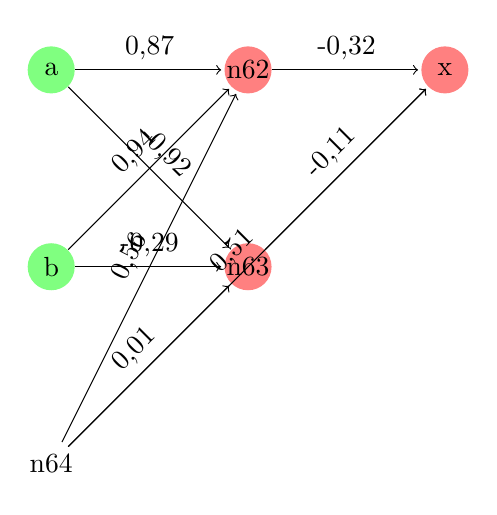
\begin{tikzpicture}[shorten >=1pt,->,draw=black!,node distance=2.5cm]
\tikzstyle{neuron}=[circle,fill=black!25,minimum size=17pt,inner sep=0pt]
\tikzstyle{constant}=[neuron, fill=white!50];
\tikzstyle{sigmoid}=[neuron, fill=red!50];
\tikzstyle{identity}=[neuron, fill=green!50];
\node [identity] (a) {a};
\node [identity,below of=a] (b) {b};
\node [constant,below of=b] (n64) {n64};
\node [sigmoid,right of=a] (n62) {n62};
\node [sigmoid,below of=n62] (n63) {n63};
\node [sigmoid,right of=n62] (x) {x};
\path[every node/.style={sloped,anchor=south,auto=false}]
(n62) edge node {-0,32} (x)
(n63) edge node {-0,11} (x)
(a) edge node {0,87} (n62)
(a) edge node {-0,92} (n63)
(b) edge node {-0,29} (n63)
(b) edge node {0,94} (n62)
(n64) edge node {0,51} (x)
(n64) edge node {0,01} (n63)
(n64) edge node {0,56} (n62)
;\end{tikzpicture}
\end{document}